% 04-rlvr: RLVR = RL where the reward comes from a programmatic verifier.
% Running example (shared with section 06): "What is 17 x 24?", answer 408, verifier -> 1 if equal else 0.

% token box for TikZ pictures: \node[s4tok=<color>] {text};
\tikzset{
  s4tok/.style={draw=#1, fill=#1!10, rounded corners=2pt, inner sep=2pt,
    text height=1.6ex, text depth=0.4ex, font=\ttfamily\scriptsize},
  s4tok/.default=gray,
  % keeps the path (and its bounding box) on every overlay, only makes it transparent before <n>
  s4alt/.code args={<#1>#2#3}{\alt<#1>{\pgfkeysalso{#2}}{\pgfkeysalso{#3}}},
  s4vis/.style={s4alt={#1{}{opacity=0}}},
  s4tag/.style={font=\scriptsize, inner sep=1pt, align=center},
}
% $\times$ inside \texttt for token boxes
\newcommand{\sfourmul}{$\times$}

\section*{RLVR}

\begin{frame}{The RLVR Loop}
  \vfill
  \centering
  \makebox[0pt][c]{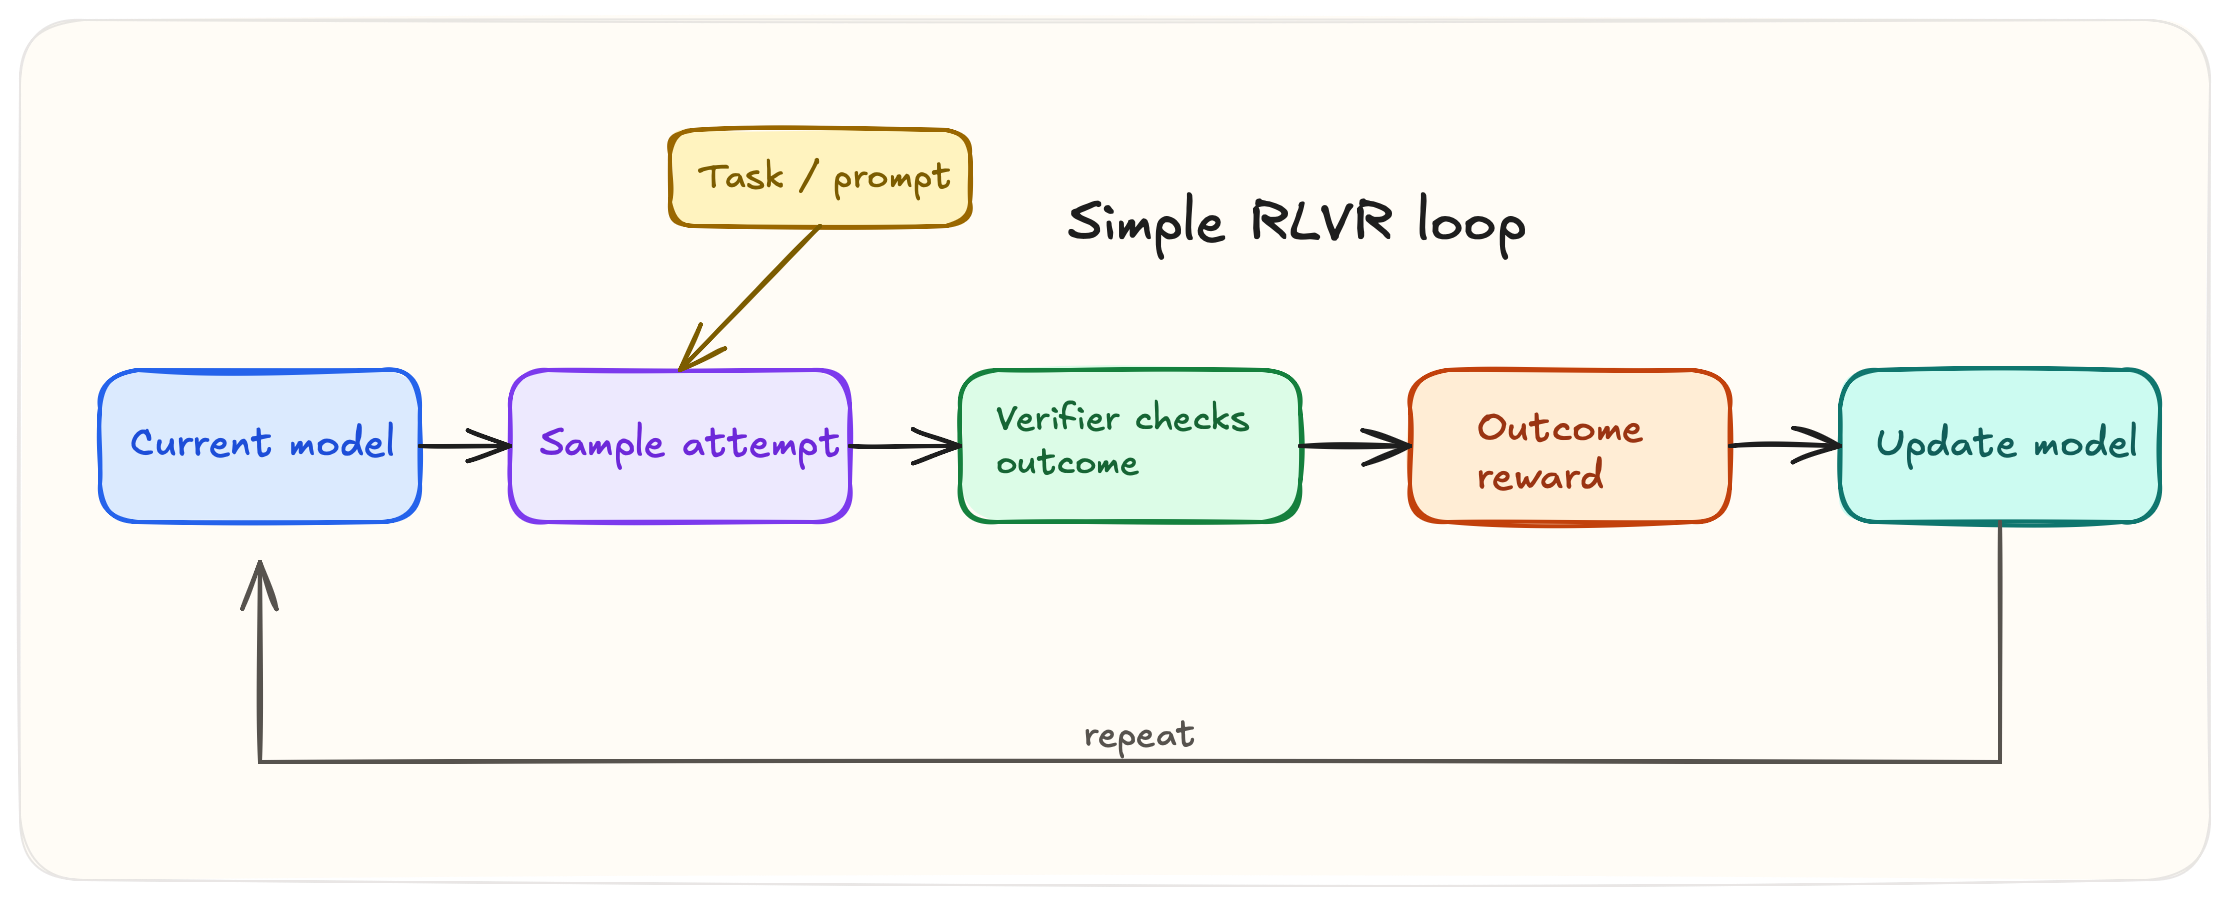
\includegraphics[width=1.14\textwidth]{01-verifier-stack-light.png}}
  \source{Figure from rlvrbook.com, Ch.~1}
  \vfill
\end{frame}

\begin{frame}{RL Concepts on an LLM}
  \vfill
  \centering
  \begin{tikzpicture}[x=1cm, y=1cm, scale=1.0, transform shape, >={Stealth[length=3pt]}]
    % prompt (environment) and response (agent) tokens, one row
    \node[s4tok=envcolor] (p0) {What};
    \node[s4tok=envcolor, right=2pt of p0] (p1) {is};
    \node[s4tok=envcolor, right=2pt of p1] (p2) {17\sfourmul 24};
    \node[s4tok=envcolor, right=2pt of p2] (p3) {?};
    \node[s4tok=agentcolor, right=8pt of p3] (r0) {17\sfourmul 24};
    \node[s4tok=agentcolor, right=2pt of r0] (r1) {=};
    \node[s4tok=agentcolor, right=2pt of r1] (r2) {408};
    \node[s4tok=agentcolor, right=2pt of r2] (r3) {<eos>};

    % <2> environment: one dashed container = prompt (top) + verifier (bottom)
    \node[s4vis=<2->, rlbox=envcolor, minimum width=2.4cm, minimum height=0.9cm] (ver)
      at ($(p0.west)!0.5!(p3.east)+(0,-1.9)$) {\textbf{verifier}\\[-1pt]\scriptsize\texttt{ans == 408?}};
    \begin{scope}[on background layer]
      \node[s4vis=<2->, draw=envcolor, dashed, rounded corners=3pt, fit=(p0)(p3)(ver), inner sep=6pt] (envbox) {};
    \end{scope}
    \node[s4vis=<2->, font=\footnotesize\bfseries, text=envcolor, rotate=90, anchor=south, inner sep=3pt] at (envbox.west) {environment};

    % <3> state: brace above the prompt + tokens so far
    \draw[s4vis=<3->, decorate, decoration={brace, amplitude=4pt}, thick, black]
      ($(p0.north west)+(0,0.1)$) -- ($(r1.north east)+(0,0.1)$)
      node[midway, above=6pt, font=\footnotesize, text=black] {state $s_t$};

    % <4> action: next token
    \node[s4vis=<4->, draw=black, very thick, rounded corners=2pt, fit=(r2), inner sep=1.5pt] (act) {};
    \node[s4vis=<4->, font=\footnotesize, align=center, text=black, below=4pt of act] (actlab)
      {action $a_t$\\[-1pt]next token\\[-1pt]$\sim$100k choices};

    % <5> policy: the LLM itself, straight above the action
    \node[s4vis=<5->, rlbox=agentcolor, minimum width=3.2cm, minimum height=0.9cm, above=1.0cm of r2] (pol)
      {\textbf{policy} = the LLM\\[-1pt]$\pi_\theta(a_t\mid s_t)$};
    \draw[s4vis=<5->, rlarrow=agentcolor] (pol.south) -- (act.north);

    % <6> reward: from <eos> to the verifier, then 0/1 below it
    \draw[s4vis=<6->, rlarrow=rewardcolor] (r3.east) -- ++(0.3,0) |- (ver.east);
    \node[s4vis=<6->, rlbox=rewardcolor, minimum width=2.4cm, minimum height=0.9cm, below=1.1cm of ver] (rew)
      {\textbf{reward}\\[-1pt]$r=1$, only at the end};
    \draw[s4vis=<6->, rlarrow=rewardcolor] (ver.south) -- (rew.north);
  \end{tikzpicture}
  \vfill
\end{frame}

\begin{frame}{Why Not Just Imitate?}
  \vfill
  \centering
  \begin{tikzpicture}[x=1cm, y=1cm, scale=1.3, transform shape, >={Stealth[length=3pt]},
      col/.style={minimum width=2.95cm, minimum height=0.95cm}]
    % left column: SFT (x = -2.4)
    \node[font=\bfseries] at (-2.4, 2.4) {Supervised (SFT)};
    \node[rlbox=humancolor, col] (sp) at (-2.4, 1.2) {prompt};
    \node[rlbox=humancolor, col] (ss) at (-2.4, 0)   {one human solution};
    \node[rlbox=humancolor, col] (sl) at (-2.4, -1.2) {copy it, token by token};
    \draw[rlarrow=humancolor] (sp) -- (ss);
    \draw[rlarrow=humancolor] (ss) -- (sl);
    % right column: RLVR (x = +2.4)
    \node<2->[font=\bfseries, text=agentcolor] at (2.4, 2.4) {RLVR};
    \node<2->[rlbox=agentcolor, col] (rp) at (2.4, 1.2) {prompt};
    \node<2->[rlbox=agentcolor, col] (rs) at (2.4, 0)   {many own samples};
    \node<2->[rlbox=envcolor, col] (rl) at (2.4, -1.2) {verifier: right or wrong?};
    \draw<2->[rlarrow=agentcolor] (rp) -- (rs);
    \draw<2->[rlarrow=envcolor] (rs) -- (rl);
    \draw<2->[gray!50, dashed] (0, 2.8) -- (0, -1.7);
  \end{tikzpicture}
  \vfill
\end{frame}

\begin{frame}{Right Answer, Different Words}
  \vfill
  \centering
  \begin{tikzpicture}[x=1cm, y=1cm, scale=1.3, transform shape, >={Stealth[length=3pt]}]
    % reference solution
    \node[s4tag, anchor=east, text=black] at (-0.1, 1.0) {human\\reference};
    \node[s4tok=humancolor, anchor=west] (h0) at (0, 1.0) {17\sfourmul 20};
    \node[s4tok=humancolor, right=2pt of h0] (h1) {=};
    \node[s4tok=humancolor, right=2pt of h1] (h2) {340};
    \node[s4tok=humancolor, right=2pt of h2] (h3) {+};
    \node[s4tok=humancolor, right=2pt of h3] (h4) {68};
    \node[s4tok=humancolor, right=2pt of h4] (h5) {=};
    \node[s4tok=humancolor, right=2pt of h5] (h6) {408};
    % model's own correct answer
    \node[s4tag, anchor=east, text=agentcolor] at (-0.1, 0) {model\\sample};
    \node[s4tok=agentcolor, anchor=west] (m0) at (0, 0) {24\sfourmul 17};
    \node[s4tok=agentcolor, right=2pt of m0] (m1) {=};
    \node[s4tok=agentcolor, right=2pt of m1] (m2) {408};
    % verdicts: two equal boxes, branching from one stem under the sample row
    \node<2->[rlbox=humancolor, minimum width=3.3cm, minimum height=1.2cm] (sv) at ($(m1.south)+(-2.0,-1.8)$)
      {\textbf{SFT loss}\\[-1pt]\textcolor{rewardcolor}{\ding{55}} differs from reference};
    \node<3->[rlbox=envcolor, minimum width=3.3cm, minimum height=1.2cm] (rv) at ($(m1.south)+(2.0,-1.8)$)
      {\textbf{verifier}\\[-1pt]408 \textcolor{envcolor}{\ding{51}}\quad $r=1$};
    \draw<2->[rlarrow=humancolor] (m1.south) -- ++(0,-0.6) -| (sv.north);
    \draw<3->[rlarrow=envcolor] (m1.south) -- ++(0,-0.6) -| (rv.north);
  \end{tikzpicture}
  \vfill
  \visible<3->{\keyidea{SFT rewards matching the teacher. RLVR rewards being right.}}
  \vfill
\end{frame}
